\documentclass[submit]{harvardml}

% FDV: Make sure all front matter has correct years, dates, book sections, etc.
\course{CS181-S23}
\assignment{Assignment \#2}
\duedate{11:59pm EST, Feb 23th, 2023}

\usepackage[OT1]{fontenc}
\usepackage[colorlinks,citecolor=blue,urlcolor=blue]{hyperref}
\usepackage{float}
\usepackage[caption = false]{subfig}
\usepackage[final]{graphicx}
\usepackage{subfig}
\usepackage{fullpage}
\usepackage{amsmath}
\usepackage{amssymb}
\usepackage{framed}
\usepackage{color}
\usepackage{soul}
\usepackage{todonotes}
\usepackage{listings}
\usepackage{common}
\usepackage{enumitem}
\usepackage{bm}
\usepackage{bbm}
\newcommand{\B}{\text{B}}
\newcommand{\Beta}{\text{Beta}}

\usepackage[mmddyyyy,hhmmss]{datetime}

\usepackage{comment}
\usepackage{url}
\usepackage{xcolor}
\usepackage{mdframed}

\definecolor{codegreen}{rgb}{0,0.6,0}
\definecolor{codegray}{rgb}{0.5,0.5,0.5}
\definecolor{codepurple}{rgb}{0.58,0,0.82}
\definecolor{backcolour}{rgb}{0.95,0.95,0.92}

\definecolor{verbgray}{gray}{0.9}

\lstnewenvironment{csv}{%
  \lstset{backgroundcolor=\color{verbgray},
  frame=single,
  framerule=0pt,
  basicstyle=\ttfamily,
  columns=fullflexible}}{}

\begin{document}

\begin{center}
{\Large Homework 2: Classification and Bias-Variance Trade-offs}\\
\end{center}

\subsection*{Introduction}

This homework is about classification, bias-variance trade-offs, and uncertainty quantification. In lecture we have primarily focused on binary classifiers trained to discriminate between two classes. In multiclass classification, we
discriminate between three or more classes. 
We encourage you to read
CS181 Textbook's Chapter 3 for more information on linear
classification, gradient descent, and classification in the discriminative setting. Read Chapter 2.8 for more
information on the trade-offs between bias and variance.

The datasets that we will be working with relate to astronomical observations. The first dataset, found at \verb|data/planet-obs.csv|, contains information on whether a planet was observed (as a binary variable) at given points in time. This will be used in Problem 1. The second dataset, available at \verb|data/hr.csv|, details different kinds of stars and their measured magnitude and temperature. You will work with this data in Problem 3.
As a general note, for classification problems we imagine that we have
the input matrix $\boldX \in \reals^{n \times d}$ (or perhaps they
have been mapped to some basis $\bm{\Phi}$, without loss of
generality) with outputs now ``one-hot encoded."  This means that if
there are~$K$ output classes, rather than representing the output
label $y$ as an integer~${1,2,\ldots,K}$, we represent $\boldy$ as a
``one-hot" vector of length~$K$. A ``one-hot" vector is defined as
having every component equal to 0 except for a single component which
has value equal to 1.  For example, if there are $K = 7$ classes and a
particular data point belongs to class 3, then the target vector for
this data point would be~$\boldy = [0,0,1,0,0,0,0]$.  We will define
$C_1$ to be the one-hot vector for the 1st class, $C_2$ for the 2nd
class, etc.  Thus, in the previous example $\boldy = C_3$. If there
are $K$ total classes, then the set of possible labels is $\{C_1
\ldots C_K \} = \{C_k\}_{k=1}^K$.  Throughout the assignment we will
assume that each label $\boldy \in \{C_k\}_{k=1}^K$ unless otherwise
specified. The most common exception is the case of binary classification
($K = 2$), in which case labels are the typical integers $y \in \{0, 1\}$.

In problems 1 and 3, you may use \texttt{numpy} or \texttt{scipy}, but
not \texttt{scipy.optimize} or \texttt{sklearn}. Example code given is
in Python 3.

Please type your solutions after the corresponding problems using this
\LaTeX\ template, and start each problem on a new page.

Please submit the \textbf{writeup PDF to the Gradescope assignment `HW2'}. Remember to assign pages for each question.  \textbf{You must include your plots in your writeup PDF. } The supplemental files will only be checked in special cases, e.g. honor code issues, etc.

Please submit your \textbf{\LaTeX\ file and code files to the Gradescope assignment `HW2 - Supplemental'}. 

%%%%%%%%%%%%%%%%%%%%%%%%%%%%%%%%%%%%%%%%%%%%%
% Problem 1
%%%%%%%%%%%%%%%%%%%%%%%%%%%%%%%%%%%%%%%%%%%%%

\begin{problem}[Exploring Bias-Variance and Uncertainty]
In this problem, we will explore the bias and variance of a few different model classes when it comes to logistic regression and investigate two sources of predictive uncertainty.

We are currently managing a powerful telescope that is being used to monitor and gather measurements of some planet of interest. At certain times however, our telescope is unable to detect the planet at all. The data in \verb|data/planet-obs.csv| records the observation time in the ``Time" column and whether the planet was detected in the ``Observed" column (with the value 1 representing that it was observed). Since it is expensive to use and maintain the telescope, we would like to build a model to help us schedule and find times when we are likely to detect the planet.

\begin{enumerate}

\item First split the data into 10 mini-datasets of size $N = 30$ (i.e. dataset 1 consists of the first 30 observations, dataset 2 consists of the next 30, etc. This has already been done for you). Consider the three bases $\boldsymbol\phi_1(t) = [1, t]$, $\boldsymbol\phi_2(t) = [1,
  t, t^2]$, and $\boldsymbol\phi_3(t) = [1, t, t^2, t^3, t^4, t^5]$. For each of these bases, fit a logistic regression model using sigmoid($\boldw^\top \boldsymbol\phi(t)$) to each dataset by using gradient descent to
  minimize the negative log-likelihood.  This means you will be
  running gradient descent 10 times for each basis, once for each
  dataset.
  
  Use the given starting values of $\boldw$ and a learning rate of $\eta=0.001$, take 10,000 update
  steps for each gradient descent run, and make sure to average the
  gradient over the data points at each step. These parameters,
  while not perfect, will ensure your code runs reasonably quickly. 

\item After consulting with a domain expert, we find that the probability of observing the planet is periodic as the planet revolves around its star---we are more likely to observe the planet when it is in front of its star than when it is behind it. In fact, the expert determines that observation follows the generating process $y \sim \text{Bern}(f(t))$, where $f(t) = 0.4 \times \cos(1.1t + 1) + 0.5$ for $t \in [0, 6]$ and $y \in \{0,1\}$. Note that we, the modelers, do not usually see the true data distribution. Knowledge of the true $f(t)$ is only exposed in this problem to allow for verification of the true bias.

Use the given code to plot the true process versus your learned models. Include your plots in your solution PDF.

\textbf{In no more than 5 sentences}, explain how bias and variance reflected in the 3 types of curves on the graphs.  How do the fits of the individual and mean prediction functions change?  Keeping in mind that none of the model classes match the true generating process exactly, discuss the extent to which each of the bases approximates the true process.

\item If we were to increase the size of each dataset drawn from $N = 30$ to a larger number, how would the bias and variance change for each basis? Why might this be the case? You may experiment with generating your own data that follows the true process and plotting the results, but this is \textbf{not} necessary. \textbf{Your response should not be longer than 5 sentences}.

\item Consider the test point $t = 0.1$. Using your models trained on basis $\boldsymbol\phi_3$, report the predicted probability of observation of the \textit{first} model (the model trained on the first 30 data points). How can we interpret this probability as a measure of uncertainty? Then, compute the variance of the classification probability over your 10 models at the same point $t = 0.1$. How does this measurement capture another source of uncertainty, and how does this differ from the uncertainty represented by the classification probability?

Repeat this process (reporting the first model's classification probability and the variance over the 10 models) for the point $t = 3.2$. At which point in time would you be more confident in detecting the planet? There's no right answer---you should consider the two different types of uncertainty and their implications when translating from model output to decision making.

\end{enumerate}
\end{problem}
 \let\cleardoublepage\clearpage

%%%%%%%%%%%%%%%%%%%%%%%%%%%%%%%%%%%%%%%%%%%%%
% Solution Problem 1
%%%%%%%%%%%%%%%%%%%%%%%%%%%%%%%%%%%%%%%%%%%%%
\newpage

\textbf{Solution 1:}

\begin{enumerate}
\item See code in jupyter notebook.
\item See the plots below:

\begin{figure}[h]
\subfloat[fig 1]{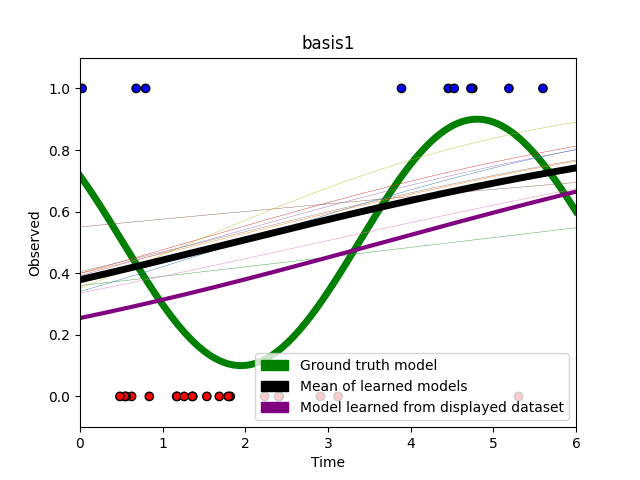
\includegraphics[width = 3in]{hw2/basis1.png}} 
\subfloat[fig 2]{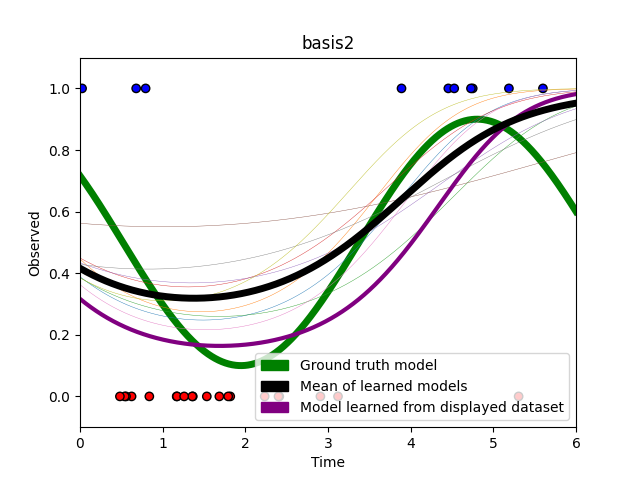
\includegraphics[width = 3in]{hw2/basis2.png}}\\
\subfloat[fig 3]{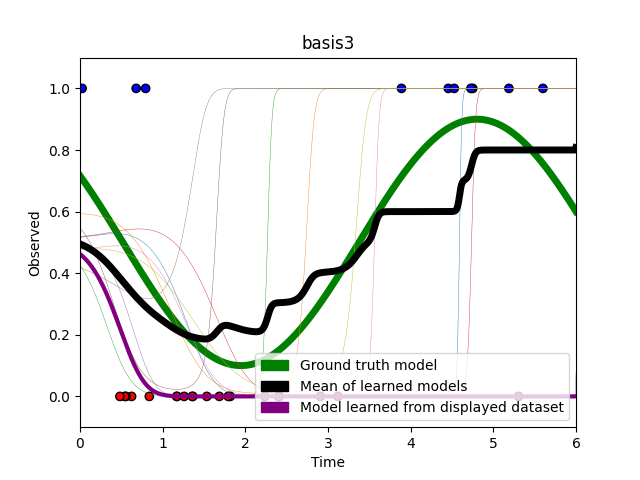
\includegraphics[width = 3in]{hw2/basis3.png}} 
\caption{Plots of different bases}
\label{fig:figure}
\end{figure}


For the first basis, the model under-fits the data, showing high bias and low variance (with transformed input matrix of only $nx2$) and completely misses the mark with the true process (all of the individual prediction functions are straight lines.) 

The second basis fits the data, more closely approximating the true process, with low bias and low variance – the mean of the individual prediction function captures the trend more generally (you can see in the graph that some of the individual ones fit better than others, depending on what part of the data-set they were trained on.) 

The third basis shows a model that clearly overfits the data (low bias, high variance). Despite being a better fit than basis one, we can see that each individual prediction function grossly overfits to the datapoints, and the mean of the prediction functions reflects that with its sudden variations.


\item Intuitively, the model would be more generalizable since there would be more data for the model to train on, and so variance would decrease. Bias 'measures the difference between the true function and our estimate $f_{\hat{w}}$ averaged over all samples of training sets' [from lecture video] and so it would be unaffected by the size of the data set.

\item Observation prob @ $t=0.1$ $\approx 0.5198$.\\
Variance of the classification probability over 10 models $\approx 0.0038$\\
The observation probability tells us that we can be about $50\%$ sure that we'll observe the planet. The variance tells us how much this probability varies across the 10 different models. Since it's very low, we can be fairly certain of this probability.

Observation prob @ $t=3.2$ $\approx 6.591e-11$\\
Variance of the classification probability over 10 models $\approx 0.2289$\\
The observation probability tells us that it's very unlikely that the planet was observed -- however, this probability varies considerably among the 10 different models.

I would be more confident in detecting the planet at $t=0.1$, because when we check the mean of each, the first test point has mean $\approx 0.4820$, compared to the second with mean $\approx 0.4171$. Since the first test point has both a higher mean and a more certain probability, I'd place my bets there.

\end{enumerate}

%%%%%%%%%%%%%%%%%%%%%%%%%%%%%%%%%%%%%%%%%%%%%
% Problem 2
%%%%%%%%%%%%%%%%%%%%%%%%%%%%%%%%%%%%%%%%%%%%%

\begin{problem}[Multi-class Logistic Regression and Softmax]
The objective of this problem is to generalize binary logistic regression into the more general case of three or more classes. You will use the results of this problem to implement a classifier in Problem 3.

Consider a $K$-class model with $K \geq 3$. Suppose we have a data set $\{(\boldx_i,
\boldy_i)\}_{i=1}^n$ with features $\{\boldx_n\}_{n = 1}^N \in \mathbb{R}^d$ and one-hot encoded outputs $\{\boldy_n\}_{n = 1}^N \in \mathbb{R}^K$ (see the introduction of this homework). For a $K$-dimensional vector $\boldz = [z_1, \dots, z_K]^\top$, define the \textit{softmax} function to be
$$
\text{softmax}(\boldz) = \frac{1}{\sum_{i = 1}^K \exp(z_i)}
\begin{bmatrix}
\exp(z_1) \\
\exp(z_2) \\
\vdots \\
\exp(z_K)
\end{bmatrix}.
$$
In other words, the softmax function is a function from $\mathbb{R}^K$ to $\mathbb{R}^K$ with $k$-th component of the output
$$
\text{softmax}_k(\boldz) = \frac{\exp(z_k)}{\sum_{i = 1}^K \exp(z_i)}.
$$
We will use the shorthand notation $s_k(\boldz)$ to abbreviate the above. Note that the softmax function is the general form of the sigmoid function in binary logistic regression. This means that the derivations in this problem will be very similar to what you have seen in class.

\begin{enumerate}
  \item For $j, k \in \{1, \dots, K\}$, show that the partial derivatives of the softmax function can be written in terms of the softmax function itself in the following form:
  $$
  \frac{\partial s_k(\boldz)}{\partial z_j} = s_k(\boldz)(\delta_{jk} - s_j(\boldz))
  $$
  Here, $\delta_{jk}$ denotes the \textit{Kronecker delta} function $\delta_{jk}$:
  $$
  \delta_{jk} = 
  \begin{cases}
    1 \text{ if } j = k, \\
    0 \text{ if } j \neq k.
  \end{cases}
  $$
  Since all of these partial derivatives are with respect to scalars, you can use the typical quotient rule from your univariate calculus class. It may help to consider the cases $j = k$ and $j \neq k$ separately.
  
  Using the answer above, find the logarithmic derivatives of $\text{softmax}(\boldz)$; that is, find $\displaystyle \frac{\partial \ln s_k(\boldz)}{\partial z_j}$ for $j, k \in \{1, \dots, K\}$.
\end{enumerate}

Multi-class logistic regression has weights $\{\boldw_j\}_{j=1}^K \in \mathbb{R}^d$ for each class, which are often condensed into a single matrix $\boldW \in \mathbb{R}^{K \times d}$ (the $j$-th row of $\boldW$ corresponds to $\boldw_j$). We model the probabilities of class membership independently as
$$
p(\boldy_n = C_k | \boldx_n, \boldW) = s_k(\boldW\boldx_n)
$$
for $k \in \{1, \dots, K\}$ and $n \in \{1, \dots, N\}$.
In addition, let $y_{nk}$ denote the $k$-th component of the output vector $\boldy_n$. 
\begin{enumerate}
    \item[2.] Write out the negative log-likelihood of the data set, $\ell(\boldW) = -\ln p(\{\boldy_n\}_{n=1}^N | \{\boldx_n\}_{n=1}^N, \boldW)$, in terms of $s_k, \boldW, \{\boldx_n\}_{n=1}^N$, and $y_{nk}$. You can start by noting that for a single observation $(\boldx_n, \boldy_n)$,
    $$
    p(\boldy_n | \boldx_n, \boldW) = \prod_{k=1}^Kp(\boldy_n = C_k | \boldx_n, \boldW)^{y_{nk}}
    $$
    because $y_{nk} = 1$ if $\boldy_n$ belongs to class $C_k$ and $y_{nk} = 0$ otherwise. The equation above simply lets us combine all possible class memberships of $\boldy_i$ into a single expression. This is also known as the ``power trick" as we express the probability as a product of terms raised to a power that is either 0 or 1.
\end{enumerate}
\end{problem}

\begin{framed}
\noindent\textbf{Problem 2} (cont.)\\
\begin{enumerate}
    \item[3.] Consider the weight matrix $\boldW$ and the $i$-th feature vector $\boldx_i$. Denote their product as $\boldz_i = \boldW\boldx_i$. Compute the derivative of $\ell(\boldW)$ with respect to the $j$-th coordinate of the $K$-dimensional vector $\boldz_i$ (denoted as $z_{ij}$). In particular, show that 
    $$
    \frac{\partial \ell}{\partial z_{ij}} = \sum_{k = 1}^K y_{ik}(s_j(\boldz_i) - \delta_{kj})
    $$
    You may want to use your answer from part 1. Then, show that the above sum can be simplified:
    $$
    \sum_{k = 1}^K y_{ik}(s_j(\boldz_i) - \delta_{kj}) = s_j(\boldz_i) - y_{ij}.
    $$
    It will help to consider the case $k = j$ separately again and remove the delta function from the equation.
    \item[4.] Conclude that the gradient of negative log-likelihood with respect to a single weight vector $\boldw_j$ is given by the \textit{vector}
    $$
    \frac{\partial \ell}{\partial \boldw_j} = \sum_{n = 1}^N(s_j(\boldW\boldx_n) - y_{nj})\boldx_n
    $$
    for $j \in \{1, \dots, K\}$. This can be done by using the chain rule:
    $$
    \frac{\partial \ell}{\partial \boldw_j} = \sum_{n = 1}^N\sum_{k = 1}^K\frac{\partial \ell}{\partial z_{nk}}\frac{\partial z_{nk}}{\partial \boldw_j}.
    $$
    We found the first derivative in part 3. What do we know about the second derivative when $k \neq j$? You can start by expressing $z_{nk}$ in terms of the vectors $\{\boldw_i\}_{i=1}^K$ and $\{\boldx_i\}_{i=1}^N$.
    
    We can use this final expression to optimize the weights via gradient descent!
\end{enumerate}
\end{framed}

%%%%%%%%%%%%%%%%%%%%%%%%%%%%%%%%%%%%%%%%%%%%%
% Solution Problem 2
%%%%%%%%%%%%%%%%%%%%%%%%%%%%%%%%%%%%%%%%%%%%%
\pagebreak

\textbf{Solution 2:}

\begin{enumerate}
\item 
Using the quotient rule, for $j \neq k$:
\begin{align*}
    \frac{\partial s_k(\bm{z})}{\partial z_j} &= \frac{\sum^K_{i=1}\exp(z_i) \cdot 0 - \exp(z_k)\cdot\exp(z_j)}{(\sum_{i=1}^K \exp(z_i))^2}\\
    &= \frac{\exp(z_k)}{\sum_{i=1}^K \exp(z_i)} \cdot \left(- \frac{\exp(z_j)}{\sum_{i=1}^K \exp(z_i)}\right)\\
    &= s_k(\boldz)(0 - s_j(\boldz))
\end{align*}

For $j=k$:
\begin{align*}
    \frac{\partial s_k(\bm{z})}{\partial z_j} &= \frac{\sum^K_{i=1}\exp(z_i) \cdot \exp(z_k) - \exp(z_k)\cdot\exp(z_j)}{(\sum_{i=1}^K \exp(z_i))^2}\\
    &= \frac{\exp(z_k)}{\sum_{i=1}^K \exp(z_i)} \cdot \left(\frac{\sum^K_{i=1}\exp(z_i) - \exp(z_j)}{\sum_{i=1}^K \exp(z_i)}\right)\\
    &= s_k(\boldz)(1 - s_j(\boldz))
\end{align*}

Using this result and the chain rule, we can find the derivative of $\ln s_k(\bm{z})$:

\begin{align*}
    \frac{\partial \ln s_k(\bm{z})}{\partial z_j} &= \frac{1}{s_k(\boldz)} \cdot s_k(\boldz)(\delta_{ij} - s_j(\boldz))\\
    &= \delta_{ij} - s_j(\boldz)
\end{align*}

\item
We have our negative log-likelihood:
\begin{align*}
    \ell(\boldW) &= -\ln p(\{\boldy_n\}_{n=1}^N | \{\boldx_n\}_{n=1}^N, \boldW)\\
    &= -\ln \prod_{n=1}^N p(\boldy_n | \boldx_n, \boldW)\\
    &= -\ln \prod_{n=1}^N \prod_{k=1}^K p(\boldy_n = C_k | \boldx_n, \boldW)^{y_{nk}}\\
    &= \sum_{n=1}^N \sum_{k=1}^K y_{nk} \ln s_k(\boldW\boldx_n) 
\end{align*}


\item 
We know that $\boldz_i = \boldW \boldx_i$. Thus, $z_{ij} = w_j x_i$ Taking the derivative of the NLL:
\begin{align*}
    \frac{\partial\ell(\boldW)}{\partial z_{ij}} = \frac{\partial\ell(\boldW)}{\partial w_j x_i} &= -\sum_{k=1}^K y_{ik} \frac{1}{s_k(\boldW\boldx_i)} \cdot s_k(\boldW\boldx_i)(\delta_{jk} - s_j(\boldW\boldx_i))\\
    &= \sum_{k=1}^K y_{ik} (s_j(\boldW\boldx_i) - \delta_{jk})\\
    &= \sum_{k=1}^K y_{ik} (s_j(\boldz_i) - \delta_{jk})\\
\end{align*}

For the term in the sum where $k=j$:

\begin{align*}
    y_{ik}(s_k(\boldz_i) - 1) = y_{ij}s_j(\boldz_i) - y_{ij} 
\end{align*}

For all other terms:

\begin{align*}
    \sum^K_{k=1, k \neq j} y_{ik}s_j(\boldz_i)
\end{align*}

Summing all of the terms together:

\begin{align*}
    \sum_{k=1}^K y_{ik} (s_j(\boldz_i) - \delta_{jk}) &= y_{ij}s_j(\boldz_i) - y_{ij} + \sum^K_{k=1, k \neq j} y_{ik}s_j(\boldz_i)\\
    &= \sum^K_{k=1} y_{ik}s_j(\boldz_i) - y_{ij}\\
    &= s_j(\boldz_i) - y_{ij}
\end{align*}

\item 
When we consider the second derivative $\frac{\partial z_{nk}}{\boldw_j}$ we see that when $j \neq k$, it evaluates to zero since $z_{nk} = \boldw_k \boldx_n$. When $j = k$, it evaluates to $x_n$. Thus, we have:

\begin{align*}
    \frac{\partial \ell}{\partial \boldw_j} &= \sum_{n=1}^N \frac{\partial \ell}{\partial z_{nk}} x_n\\
    &= \sum_{n=1}^N (s_j(\boldz_n) - y_{nj})x_n
\end{align*}

\end{enumerate}
%%%%%%%%%%%%%%%%%%%%%%%%%%%%%%%%%%%%%%%%%%%%%
% Problem 3
%%%%%%%%%%%%%%%%%%%%%%%%%%%%%%%%%%%%%%%%%%%%%

\begin{problem}[Classifying Stars]
In this problem, you will code up three different classifiers to classify different types of stars. The file \verb|data/hr.csv| contains data on magnitude and temperature. The data can be plotted on these two axes:
\begin{center}
\includegraphics[width=.5\textwidth]{images/star.png}
\end{center}

Please implement the following classifiers in the \verb|SoftmaxRegression| and \verb|KNNClassifier| classes:

\begin{enumerate}[label=\alph*)]

\item \textbf{A multi-class logistic regression classifier} using the softmax activation function, which you investigated in Problem 2. In your implementation of gradient descent, \textbf{make sure to include a bias term and use L2 regularization} with regularization parameter $\lambda = 0.001$. Limit the number of iterations of gradient descent to 200,000, and set the learning rate to be $\eta = 0.001$.

\item \textbf{Another multi-class logistic regression classifier} with feature map $\phi(\boldx) = [\ln (x_1 + 10), x_2^2]^\top$, where $x_1$ and $x_2$ represent the values for magnitude and temperature, respectively.

\item \textbf{A kNN classifier} in which you classify based on the $k = 1$ and $k = 5$ nearest neighbors and the following distance function: $$dist(star_1, star_2) = (mag_1 - mag_2)^2/9 + (temp_1 - temp_2)^2$$
where nearest neighbors are those with the smallest distances from a given point.

  Note 1: When there are more than two labels, no label may have the
  majority of neighbors.  Use the label that has the most votes among
  the neighbors as the choice of label. 

  Note 2: The grid of points for which you are making predictions
  should be interpreted as our test space.  Thus, it is not necessary
  to make a test point that happens to be on top of a training point
  ignore itself when selecting neighbors.

\end{enumerate}

After implementing the above classifiers, complete the following exercises:

\begin{enumerate}
    \item Plot the decision boundaries generated by each classifier for the dataset. Include them in your PDF. 
    Identify the similarities and differences among the classifiers. What explains the differences---in particular, which aspects or properties of each model dictate the shape of its decision boundary? 
    
    \item 
    
    Consider a star with Magnitude 3 and Temperature -2. To which class does each classifier assign this star? Report the classification probabilities of this star for each model. 
    
    Interpret how each model makes its classification decision. What are the pros and cons of each interpretation? What else should we, the modelers, be aware of when making predictions on a test point ``far" from our training data? \textbf{Your response should no be longer than 5 sentences.}
\end{enumerate}
\end{problem}

%%%%%%%%%%%%%%%%%%%%%%%%%%%%%%%%%%%%%%%%%%%%%
% SOLUTION: Problem 3
%%%%%%%%%%%%%%%%%%%%%%%%%%%%%%%%%%%%%%%%%%%%%
\newpage

\textbf{Solution 3}

\begin{enumerate}
\item
\begin{figure}[h]
\subfloat[Softmax Regression Result]{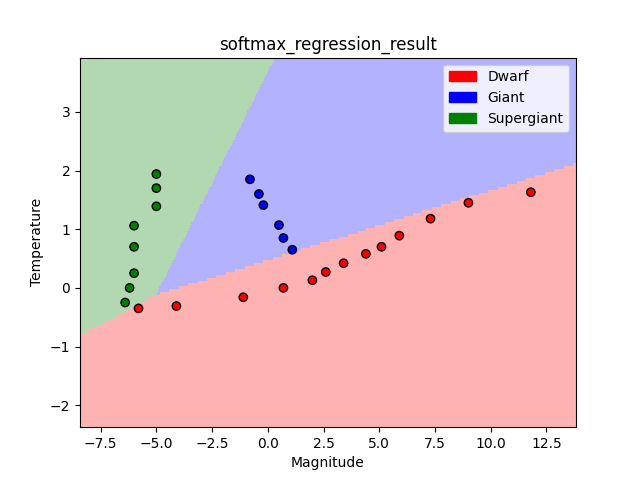
\includegraphics[width = 3in]{hw2/softmax_regression_result.png}} 
\subfloat[Basis Result]{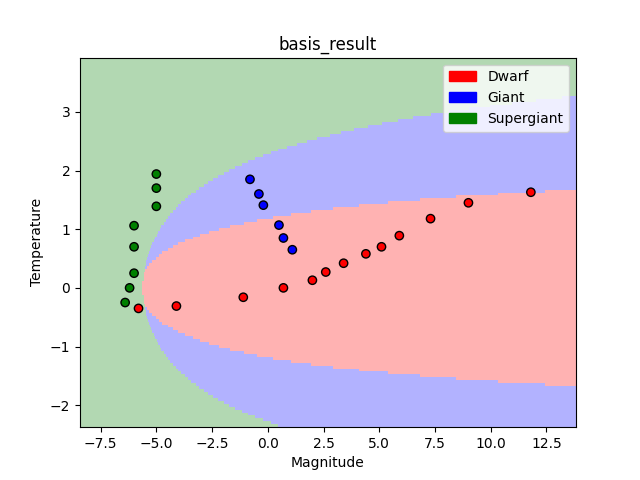
\includegraphics[width = 3in]{hw2/basis_result.png}}\\
\subfloat[KNN1 Result]{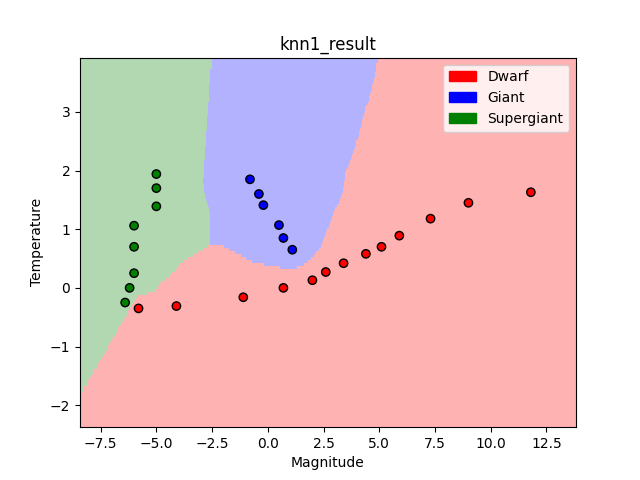
\includegraphics[width = 3in]{hw2/knn1_result.png}}
\subfloat[KNN5 Result]{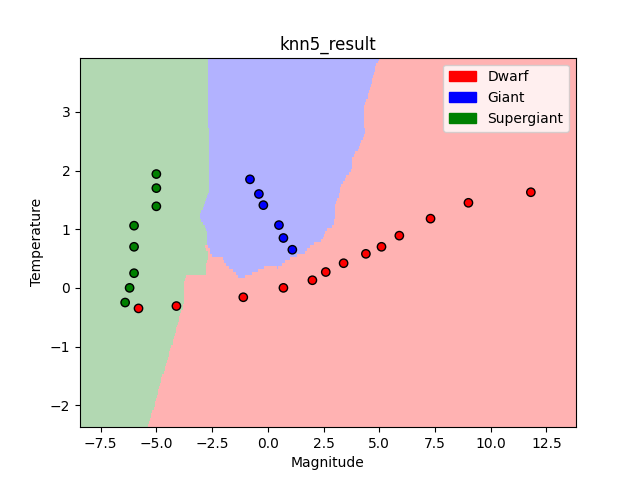
\includegraphics[width = 3in]{hw2/knn5_result.png}}
\caption{Plots decision boundaries for classifiers a, b and c}
\label{fig:problem_3_1}
\end{figure}

The vanilla and transformed basis softmax models have distinctly different boundaries, despite both being regression models–vanilla model has straight lines, which makes sense since it uses linear, non-transformed features. The transformed basis model's decision boundaries reflect the nonlinear functions in the feature map $\phi(\boldx) = [\ln(x_1 + 10), x_2^2]^T$, which cause the curved shape of the boundaries (the second covariate being squared gives rise to the parabolic-looking class boundary). Both models have similar points of intersection for the decision boundaries. 

The KNN boundaries are based on the nearest neighbours, and for both $k=1$ and $k=5$, we have a similar shape. It's clear that $k=1$ has a smoother shape, since we are only looking at the nearest neighbour to make a prediciton. For $k=5$, the boundary has a lot more variation, since it is being pulled to wherever there is a high density of points.

\item 
We compute the following predictions and prediction probabilities for $(3, -2)$:

\begin{itemize}
    \item Vanilla Softmax: Dwarf (class 0) with probabilities [1.0 1.318e-28 2.568e-40]
    \item Basis Softmax: Giant (class 1) with probabilities [0.0342 0.965 0.00119]
    \item KNN-1: Dwarf (class 0) with all neighbours class 0
    \item KNN-5: Dwarf (class 0) with all neighbours class 0
\end{itemize}

Each model generates its decision on an input based on the boundaries that it fits to the training data. If the model approximates the ground-truth model, then our generated decision will be an accurate approximation -- i.e. if there is a linear relationship between the covariates and the output, it might be reasonable to be confident in our linear model's predictions. However, when it comes to making predictions on test points that are ``far'' from the training data, we should be aware that: in the case of a linear/non-linear model, even if it is appropriate for the training data, it might not be for data that is far away (for example, a mixture model might be more appropriate); in the case of KNN model, it might not be generalizable to data that is far away from the training data, and we should be less confidence in our predictions.

\end{enumerate}

%%%%%%%%%%%%%%%%%%%%%%%%%%%%%%%%%%%%%%%%%%%%%
% Problem 4
%%%%%%%%%%%%%%%%%%%%%%%%%%%%%%%%%%%%%%%%%%%%%

\begin{problem}[Impact Question: Understanding model-assisted decision making, uncertainty in classification and model interpretation in a high-stakes situation]

\textbf{Prompt:} A pharmaceutical drug company is conducting a clinical drug trial for a devastating disease for which conventional treatment is often ineffective. They want to estimate the effectiveness of a new drug on patients in order to obtain FDA approval and release the drug to the market. They approach you with the results of their clinical trial conducted on 100 patients with features and labels as follows:

Features = \{\textit{age, sex, height, blood pressure, drug administered?}\} \\
Label = \{\textit{Did the patient get cured?}\}

Since testing on a larger patient population is expensive for various reasons, they are interested in developing a machine learning model that will estimate the effectiveness of the drug. They provide you with covariate values of a single unseen patient for testing model performance. 

\begin{enumerate}
    \item You fit a logistic regression model on the 100 observations from the clinical trial and obtain the following coefficients which minimize the negative log likelihood. Let us call this model A:

    $p(y=1 | \mathbf{x}) = \sigma(0.2 + 0.8 *\text{\textit{drug administered?}} - 0.012 *\text{\textit{age}} + 0.45*\text{\textit{sex}} +  0.001*\text{\textit{height}} - 0.007*\text{\textit{blood pressure}})$

    Say you have a female (coded as 0) patient who is age 50, 168cm tall, blood pressure 140. What is the change in classification probability of the patient getting cured when they are administered the drug versus not (please show your work)?  Use your answer to formulate an interpretation of the value of $w_1$ -- the coefficient for \textit{drug administered?} -- for stakeholders in the drug company. The drug company wants you to answer whether or not you see evidence for the efficacy of their drug -- what would you say?

    \item The drug company wants to know you how confident you are that you have the right model, so you decide to sample the existing dataset with replacement to train 100 bootstrapped models. Upon testing these 100 models on the unseen patient, you find that the predictive interval of the classification probability is around $\pm 0.35$ averaged over the bootstrapped models. The drug company is concerned and asks you to check if you can choose alternative models that are more confident in their predictions:
    \begin{enumerate}
        \item You first try adding some interaction terms and train this new model B on the original dataset:

        $p(y=1 | \mathbf{x}) = \sigma(-2 + 5*\text{\textit{drug administered?}} + 2*\text{\textit{age}} - 3.3*\text{\textit{sex}} + 0.001*\text{\textit{height}} + 0.2*\text{\textit{blood pressure}} - 0.12*\text{\textit{age}}*\text{\textit{sex}} -0.34*\text{\textit{height}}*\text{\textit{sex}})$

        Bootstrapping model B 100 times gives you a new predictive interval of $\pm 0.1$ (averaged over bootstrapped models). Why might this be happening -- how would you explain this reduction in uncertainty in model B?

        \item Encouraged by the success of adding interaction terms, you add all possible combinations of interaction terms, repeat the exercise of bootstrapping 100 times and call this model C. This gives you a predictive interval of $\pm 0.39$ averaged over the bootstrapped models. Why might this be happening -- what is the source of this rise in uncertainty? What is a solution to reduce this comparatively large uncertainty, if you wished to keep all the new terms? 
        
        \item Which model (B or C, assuming you can reduce the predictive interval for model C) would you recommend to the drug company and why?
        
    \end{enumerate}

    \item Assume that the drug company has picked model B as their final model of choice because it seems the most confident in its predictions.
    \begin{enumerate}
        \item Suppose that the confidence interval of your estimate of $w_1$ ( coefficient for $drug$ $administered?$) is $\pm 6$. What would you recommend to a critically ill patient who is desperately seeking access to this new (and very expensive, not-covered-by-insurance) drug and why?
        \item The drug company has strong reasons to believe that the drug is indeed effective. What can the drug company do during the clinical trial to tighten the confidence interval of $w_1$?
    \end{enumerate}

\end{enumerate}
\end{problem}

\begin{framed}
\noindent\textbf{Problem 4} (cont.)\\
\begin{enumerate}
\item[3.] (Continued...)
     \begin{enumerate}
     \item[(c)] From prior clinical trials and modeling efforts, the drug company scientists strongly believe that the real value of $w_1$ is either 5 or 1. For now, you take this information as ground truth. In which scenario ($w_1=1$ or $w_1=5$) is it more costly to run the drug trial and demonstrate the effectiveness of the drug? Why?\\
        \textit{Hint:} In which case do you need your confidence intervals for the estimates of $w_1$ to be tighter, to demonstrate drug effectiveness?
        \item[(d)] How do you think we should make use of domain knowledge provided by our partners -- that the real value of $w_1$ is either 5 or 1 -- during model building? For example, would it be a good idea for us to simply fix the parameter $w_1$ to be 5 or 1?
    \end{enumerate}
\item[4.] Let us revisit the data collection process during the clinical trial and consider data collected from two recruitment protocols. In the first recruitment protocol, the drug company publicly advertised the development of this drug to a hospital, encouraging interested patients to sign up for the trial. Among an audience of 100, 50 patients agreed to be administered the drug and 50 choose to opt out and are observed in the study without administering the drug. In the second recruitment protocol, the company was referred 100 patients who have the disease and administered the drug to each patient randomly based on a coin flip. When you train model B on the first dataset, it has a high value of $w_1$ and a small confidence interval of this estimate. In contrast, when you train model B on the second dataset, you get a smaller value for $w_1$ with an equally small confidence interval. Which model would you trust to predict the probability of being cured from the disease given a randomly selected new patient from a Boston hospital? Why?
\textit{Hint:} What confounding factor might we have here?

\end{enumerate}
\end{framed}

%%%%%%%%%%%%%%%%%%%%%%%%%%%%%%%%%%%%%%%%%%%%%
% Solution Problem 4
%%%%%%%%%%%%%%%%%%%%%%%%%%%%%%%%%%%%%%%%%%%%%
\newpage

\textbf{Solution 4:}

\begin{enumerate}
\item 
We have the following classification probabilities:
For \emph{drug administered}$=1$:
\begin{align*}
    p(y=1|x) = \sigma(0.2 + 0.8 * 1 - 0.012 * 50 + 0.45 * 0 + 0.001 * 168 - 0.007 * 140) \approx 0.40
\end{align*}
For \emph{drug administered}$=0$:
\begin{align*}
    p(y=1|x) = \sigma(0.2 + 0.8 * 0 - 0.012 * 50 + 0.45 * 0 + 0.001 * 168 - 0.007 * 140) \approx 0.23
\end{align*}

The change in classification probability is 0.17, which tells us that taking the drug increases the likelihood of being cured. However, since the estimate of $w_1$ is based only on 100 observations, it is not conclusive whether the drug is generally effective.

\item 
\begin{enumerate}
    \item Model B's reduced uncertainty could be explained by the possibility that there is a more complicated relationship between the predictors and the outcome, and the interaction terms could capture that complexity (compared to Model A, which shows a linear and independent relationship between the predictors and the outcome.)

    \item The rise in uncertainty could be attributed to having a highly complex model overfitting to each bootstrapped sample, resulting in high variance over the different bootstrap models. To account for this, we might add a regularization term to reduce overfitting, and/or train over a larger set of data to help our model generalize better.

    \item When it comes to the body, different factors are often interlinked, and so I'm more inclined towards Model C, since it might better capture nuances in the relationships between different factors. This is under the assumption that it is possible to reduce the predictive interval -- if it wasn't, then Model B would be a better bet, since variability is especially undesirable in healthcare contexts.
\end{enumerate}

\item 
\begin{enumerate}
    \item With a confidence interval of $\pm 6$, I would not recommend it to the patient, since (price of the medication aside) there is a chance that it would have a negative impact on them, and given that they are already critically-ill, I would not advise they take that risk. Of course, being critically-ill, they may not be able to afford time/patience, but if it is possible, I would recommend they wait till there is more conclusive information about its effects and efficacy.

    \item It could increase the sample size and diversify the data set to get a tighter confidence interval and improve its generalizability.

    \item It would be more costly for $w_1 = 1$, since the confidence intervals would need to be a lot tighter (too high of a confidence interval would indicate that a possible negative impact by taking the medicine) and we would not want to negatively impact anyone in the drug trial process.

    \item Using domain knowledge is important as it informs our decisions when we make and evaluate our models. For the real value of $w_1$, we should use them as benchmarks/goals for how accurate our model is. However, it might be a good idea not to set them, as there is always room for improvement, and by working towards getting a model that can capture the true value through training, we may end up with a stronger model–by fixing it from the start, we lose the potential of having a benchmark to evaluate our model against.
\end{enumerate}

\item
Here, our confounding factor is people having the choice of administering the drug in the first recruitment protocol. For example, patients who actively sought out and signed up for the trial may also be taking other measures to help cure the disease, and so the result of being cured may have been influenced by other factors besides the actual medication. Thus, I'd be more trusting of the model trained on the second dataset, since that recruitment protocol gets rid of those confounding factors with the patients being referred to the company, and randomly selected for having the drug administered.

\end{enumerate}


\newpage
%%%%%%%%%%%%%%%%%%%%%%%%%%%%%%%%%%%%%%%%%%%%%
% Name and Calibration
%%%%%%%%%%%%%%%%%%%%%%%%%%%%%%%%%%%%%%%%%%%%%
\subsection*{Name}
Adam Mohamed

\subsection*{Collaborators and Resources}
Evan Jiang, Taj Gulati

\subsection*{Calibration}
This pset took $~10$ hours


\end{document}
